\chapter{LANDASAN TEORI}

\section{Tinjauan Pustaka}
Penelitian ini menggunakan beberapa teori dasar supaya memperjelas proses penelitian dan memberikan pemahaman lebih lanjut. Peneltian terdahulu mengenai evaluasi performa Hadoop dan Spark dapat dilihat pada Tabel \ref{table:penelitian-dulu}.

\begin{table}[h]
\caption{Penelitian Terdahulu}
\label{table:penelitian-dulu}
\scriptsize
\begin{tabularx}{\textwidth}{c*{5}{>{\raggedright\arraybackslash}X}}
\toprule
\textbf{Tahun} & \textbf{Judul} & \textbf{Penulis} & \textbf{Metode} 
  & \textbf{Deskripsi Penelitian} \\
\midrule
2020 & \textit{A comprehensive performance analysis of Apache Hadoop and Apache Spark for large scale data sets using HiBench \cite{ahmedComprehensivePerformanceAnalysis2020}} 
  & N. Ahmed, Andre L. C. Barczak, Teo Susnjak, Mohammed A. Rashid
  & Penelitian ini menyelidiki parameter-parameter yang paling berdampak, yaitu \textit{input splits}, dan \textit{shuffle}, untuk membandingkan kinerja antara Hadoop dan Spark, dengan menggunakan klaster yang diimplementasikan di laboratorium. Guna mengevaluasi kinerja, dua beban kerja dipilih, yakni \textit{WordCount} dan  \textit{TeraSort}. Metrik kinerja diukur berdasarkan tiga kriteria: waktu eksekusi, \textit{throughput}, dan \textit{speedup}. 
  & Kinerja kedua sistem sangat bergantung pada ukuran data masukan dan pemilihan parameter yang tepat. Analisis hasil menunjukkan bahwa Spark memiliki kinerja yang lebih baik dibandingkan dengan Hadoop ketika set data kecil, mencapai peningkatan kecepatan hingga dua kali lipat dalam beban kerja \textit{WordCount} dan hingga 14 kali lipat dalam beban kerja \textit{TeraSort} ketika nilai parameter \textit{default} dikonfigurasi ulang. \\
2020 & Perbandingan Kinerja Komputasi Hadoop dan Spark untuk Memprediksi Cuaca (Studi Kasus: \textit{Storm Event Database} \cite{saputroPerbandinganKinerjaKomputasi2020}) 
  & Rendiyono Wahyu Saputro, Aminuddin, Yuda Munarko 
  & Mengimplementasikan gugus komputer untuk memproses dataset dengan berbagai ukuran dan dalam jumlah komputer yang berbeda. 
  & Hadoop memerlukan waktu yang lebih sedikit dibandingkan dengan Spark. Hal tersebut karena nilai \textit{throughput} dan \textit{throughput/node} Hadoop lebih tinggi daripada Apache Spark. \\
2018 & \textit{Performance comparison between Hadoop and Spark frameworks using HiBench benchmarks \cite{samadiPerformanceComparisonHadoop2018}} 
  & Yassir Samadi, Mostapha Zbakh, Claude Tadonki 
  & Perbandingan kinerja diimplementasikan pada mesin virtual (VM). Untuk membandingkannya, digunakan HiBench. Perbandingan dilakukan berdasarkan tiga kriteria: waktu eksekusi, \textit{throughput}, dan speedup. Beban kerja \textit{WordCount} diuji dengan ukuran data yang berbeda.
  & Spark lebih efisien dibandingkan Hadoop dalam menangani jumlah data yang besar. Namun, Spark memerlukan alokasi memori yang lebih tinggi, karena memuat data yang akan diproses ke dalam memori dan menyimpannya dalam cache untuk sementara. \\
\bottomrule
\end{tabularx}
\end{table}

\begin{table}[ht]
\caption{Lanjutan Penelitian Terdahulu}
\label{table:penelitian-dulu-lanjutan}
\scriptsize
\begin{tabularx}{\textwidth}{c*{5}{>{\raggedright\arraybackslash}X}}
\toprule
\textbf{Tahun} & \textbf{Judul} & \textbf{Penulis} & \textbf{Metode} 
  & \textbf{Deskripsi Penelitian} \\
\midrule
 2015 & \textit{Comparing Apache Spark and Map Reduce with Performance Analysis using K-Means \cite{gopalaniComparingApacheSpark2015}} 
  & Satish Gopalani, Rohan Arora
  & Hadoop dan Spark dibandingkan menggunakan algoritma pembelajaran mesin (K-Means). Ukuran data yang digunakan adalah sebesar 64MB, 1240MB dengan satu node, dan 1240MB dengan dua node.  
  & Hasil-hasil penelitian dengan jelas menunjukkan bahwa kinerja Spark jauh lebih tinggi dari segi waktu, di mana setiap ukuran dataset mengakibatkan penurunan waktu pemrosesan hingga tiga kali lipat dibandingkan dengan Hadoop. \\
\bottomrule
\end{tabularx}
\end{table}


%\begin{table}[h]
%  \centering
%  \caption{Penelitian Terdahulu}
%  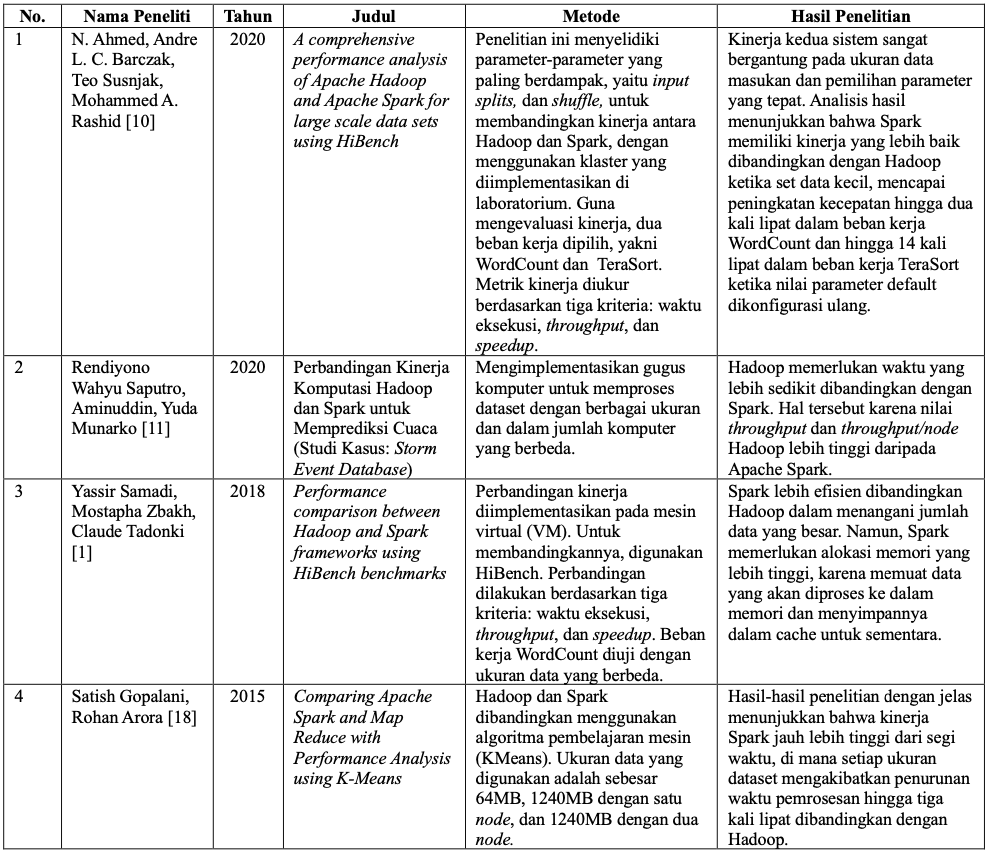
\includegraphics[width=1\textwidth]{figures/ch02/comparison-thesis}
%  \label{table:penelitian-dulu}
%\end{table}

\section{Konsep \textit{Big Data}}
\textit{Big Data} biasanya sering didefinisikan bersama dengan kompleksitas suatu data \cite{barosenAnalysisComparisonInterfacing2018}. Berbeda dengan tradisional data, \textit{Big Data} merujuk pada pertumbuhan data dalam berbagai format, baik dari struktur, semi-terstruktur, dan tidak terstruktur \cite{oussousBigDataTechnologies2018}. \textit{Big Data} memiliki banyak jenis sehingga membutuhkan teknologi yang lebih bertenaga serta algoritma yang lebih canggih. Pendekatan teknologi yang sering digunakan oleh \textit{Business Intelligence} biasanya tidak dapat lagi efisien jika digunakan.

\textit{Big Data} biasanya didefinisikan menjadi tiga karakteristik (3V), yaitu \textit{Volume, Velocity}, dan \textit{Variety} \cite{furhtIntroductionBigData2016}. \textit{Volume} berkaitan dengan jumlah data yang terbentuk atau dibuat secara terus menerus oleh beragam  perangkat, seperti telepon genggam dan aplikasi (sosial media, sensor, IoT). Jumlah data diharapkan tumbuh 5x lipat pada tahun 2020 \cite{furhtIntroductionBigData2016}. Selanjutnya, \textit{Velocity} memberikan makna bahwa data bertumbuh secara cepat dan harus diproses secara cepat juga untuk memberikan informasi yang berguna \cite{sandhuBigDataCloud2022}. YouTube adalah ilustrasi yang tepat untuk menggambarkan bagaimana pertumbuhan data begitu cepat. Terakhir, \textit{Variety} berkaitan dengan variasi sumber dan format data. 

Penerapan dari \textit{big data} tidak hanya terbatas pada pengumpulan dan penyimpanan data, tetapi juga meliputi analisis dan pengolahan data tersebut untuk menghasilkan wawasan yang berguna. Beberapa sektor yang telah menerapkan \textit{big data} secara luas meliputi kesehatan, keuangan, ritel, dan pemerintahan \cite{oussousBigDataTechnologies2018}. Dalam sektor kesehatan, \textit{big data} digunakan untuk menganalisis informasi pasien secara massal guna meningkatkan kualitas perawatan dan menemukan pola-pola penyakit. Sementara itu, di sektor keuangan, big data membantu dalam analisis risiko, deteksi penipuan, dan personalisasi layanan untuk pelanggan.

\section{Statistika Deskriptif}
Statistika deskriptif merupakan cabang statistika yang fokus pada pengorganisasian, penyajian, dan pengikhtisaran data \cite{rossIntroductoryStatistics2017}. Informasi yang diperoleh dari statistika deskriptif berguna untuk mendapatkan gambaran umum mengenai data dan untuk memahaminya secara lebih mendalam. Beberapa ukuran statistika deskriptif yang umum digunakan antara lain,

\begin{enumerate}
\item Maksimum (Max)

Maksimum (Max) merupakan nilai tertinggi dalam suatu kumpulan data. 

\begin{equation}
\text{Max} = \text{Nilai tertinggi dalam data}
\end{equation}

\item Minimum (Min)

Minimum (Min) merupakan nilai terendah dalam suatu kumpulan data. 

\begin{equation}
\text{Min} = \text{Nilai terendah dalam data}
\end{equation}

\item Rata-rata (Mean)

Rata-rata (Mean) merupakan nilai tengah dari suatu kumpulan data. Didefinisikan sebagai jumlah semua nilai data dibagi dengan jumlah total data.

\begin{equation}
\text{Mean} = \bar{x} = \frac{\sum_{i=1}^{n} x_i}{n}
\end{equation}

Keterangan:
\begin{itemize}
\item $\bar{x}$ adalah mean
\item $x_i$ adalah nilai data ke-i
\item $n$ adalah jumlah total data
\end{itemize}

\item Standar Deviasi (Std)

Standar deviasi (Std) merupakan ukuran penyebaran data terhadap mean. Semakin besar standar deviasi, semakin tersebar data dari mean. 

\begin{equation}
\text{Std} = s = \sqrt{\frac{\sum_{i=1}^{n} (x_i - \bar{x})^2}{n}}
\end{equation}

Keterangan:
\begin{itemize}
\item $s$ adalah standar deviasi
\item $x_i$ adalah nilai data ke-i
\item $\bar{x}$ adalah mean
\item $n$ adalah jumlah total data
\end{itemize}

\end{enumerate}

\section{Ekstraksi Fitur Teks (\textit{Text Feature Extraction})}
\textit{Ekstraksi Fitur Teks} adalah salah satu proses pada pembelajaran mesin (\textit{machine learning)} dan data analisis yang melibatkan identifikasi dan ekstraksi fitur yang relevan dari data mentah \cite{vijayakumarFusionBasedFeature2021}. Fitur-fitur tersebut nantinya akan digunakan untuk membuat data yang lebih informatif, sehingga dapat digunakan untuk klasifikasi, prediksi, dan klasterisasi. Ekstraksi fitur bertujuan untuk mengurangi kompleksitas data (atau yang sering disebut juga \textit{Data Dimensionality}) namun tetap menyimpan sebanyak mungkin informasi yang paling relevan. Hal ini bertujuan untuk meningkatkan performa dan efisiensi algoritma pada pembelajaran mesin dan mempermudah dalam proses analisis. Ekstraksi fitur dapat melibatkan membuat fitur baru (\textit{Feature Engineering}) atau memanipulasi data yang menghasilkan fitur yang berguna.
Ekstraksi fitur juga memainkan peran penting dalam banyak penerapan di dunia nyata, misalnya untuk pemrosesan teks dan \textit{Natural Language Processing} (NLP). Dalam skenario ini, data mentah mungkin mengandung banyak fitur yang tidak relevan atau berlebihan. Hal ini menyulitkan algoritma untuk memproses data secara akurat. Dengan melakukan ekstraksi fitur, fitur yang relevan dipisahkan dari fitur yang tidak relevan \cite{shakerFeatureExtractionBased2022}. Dengan lebih sedikit fitur yang harus diproses, kumpulan data menjadi lebih sederhana dan akurasi serta efisiensi analisis meningkat.

\subsection{\textit{Bag of Words} (BoW)}
BoW adalah teknik sederhana yang mengabaikan urutan dan struktur gramatikal kalimat, dan hanya berfokus pada frekuensi kemunculan kata dalam dokumen. Prosesnya melibatkan langkah-langkah berikut:

\begin{enumerate}
    \item \textbf{Tokenisasi:} Teks dipecah menjadi kata-kata individual (token).
    \item \textbf{Pembuatan Kosakata:} Daftar unik dari semua token yang ada dalam seluruh kumpulan dokumen dibuat. Ini disebut "kosakata".
    \item \textbf{Penghitungan Kata (Word Count): } Untuk setiap dokumen, frekuensi kemunculan setiap kata dalam kosakata dihitung. 
    \item \textbf{Representasi Vektor:} Setiap dokumen diwakili sebagai vektor, di mana setiap elemen vektor mewakili frekuensi kata tertentu dalam kosakata.
\end{enumerate}

BoW mudah diimplementasikan dan efisien, namun kelemahannya adalah kehilangan informasi kontekstual dan semantik. Kata-kata dengan frekuensi tinggi, meskipun kurang informatif, dapat mendominasi representasi vektor.

\subsection{\textit{Term Frequency-Inverse Document Frequency} (TF-IDF)}

TF-IDF mengatasi beberapa kelemahan BoW dengan mempertimbangkan pentingnya kata dalam dokumen dan koleksi dokumen \cite{qaiserTextMiningUse2018}. TF-IDF terdiri dari dua komponen:

\begin{enumerate}
    \item \textbf{\textit{Term Frequency} (TF): } Mengukur seberapa sering suatu kata muncul dalam dokumen.
    \item \textbf{\textit{Inverse Document Frequency} (IDF): } Mengukur seberapa penting suatu kata dalam seluruh koleksi dokumen. Kata-kata yang muncul di banyak dokumen (seperti kata "yang") memiliki IDF rendah, sementara kata-kata yang jarang muncul (dan kemungkinan lebih informatif) memiliki IDF tinggi.
\end{enumerate}

Dengan mengalikan TF dan IDF, kita mendapatkan nilai TF-IDF yang mencerminkan pentingnya kata dalam dokumen dan koleksi dokumen. Rumus umum untuk TF-IDF sebagai berikut, 

\begin{equation}
w_{ij} = tf_{ij} \times \log \left(\frac{N}{df_i}\right)
\end{equation}

Keterangan:

\begin{itemize}
    \item $w_{ij}$ adalah bobot tf-idf untuk kata $i$ dalam dokumen $j$;
    \item $tf_{ij}$ adalah frekuensi kemunculan kata $i$ dalam dokumen $j$ dibagi dengan total jumlah kata dalam dokumen $j$;
    \item $N$ adalah total jumlah dokumen dalam korpus;
    \item $df_i$ adalah jumlah dokumen dalam korpus yang mengandung kata $i$.
\end{itemize}

Sebagai contoh, misalkan kita ingin menghitung bobot TF-IDF untuk kata “\textit{British}” yang muncul 5 kali dalam sebuah dokumen yang berisi 100 kata. Dengan korpus yang berisi 4 dokumen, dimana 2 dokumen menyebutkan kata “British”, TF-IDF dapat dihitung sebagai berikut:

\begin{equation}
w_{British} = \frac{5}{100} \times \log \left(\frac{4}{2}\right) = 0.015
\end{equation}

TF-IDF meningkat seiring dengan peningkatan frekuensi kemunculan kata dalam dokumen, tetapi menurun seiring dengan peningkatan jumlah dokumen lain dalam korpus yang juga mengandung kata tersebut. Variasi dari skema pembobotan TF-IDF sering digunakan oleh mesin pencari sebagai alat utama dalam menilai dan meranking relevansi dokumen terhadap query pengguna.

\subsection{Penggunaan \textit{Word Count} dan \textit{Sort} pada BoW dan TF-IDF}

\begin{enumerate}
    \item \textbf{\textit{Word Count:}} Digunakan dalam kedua metode (BoW dan TF-IDF) untuk menghitung frekuensi kemunculan kata dalam dokumen.
    \item \textbf{\textit{Sort:}} Biasanya tidak digunakan secara langsung dalam proses BoW atau TF-IDF. Namun, pengurutan dapat digunakan untuk:
    \begin{itemize}
        \item \textbf{Memilih fitur:} Memilih fitur dengan nilai TF-IDF tertinggi untuk mengurangi dimensi data dan fokus pada kata-kata yang paling informatif. 
        \item \textbf{Visualisasi:} Mengurutkan kata berdasarkan frekuensi atau nilai TF-IDF dapat membantu dalam visualisasi dan analisis data.
    \end{itemize}
\end{enumerate}

\section{Komputasi Awan \textit{(Cloud Computing)}}
Komputasi awan didefinisikan sebagai sistem informasi yang memungkinkan akses mudah ke sumber daya komputasi atau layanan komputasi sesuai permintaan (\textit{on demand}), misalnya segala sesuatu mulai dari aplikasi (Google Mail, Microsft One Drive, Siakad Itera) hingga pusat data di seluruh internet dengan sistem bayar sesuai penggunaan.
Sistem komputasi awan saat ini menyediakan tiga layanan utama:
\begin{enumerate}
	\item \textit{Infrastructure as a service} (IaaS), adalah layanan awan yang menawarkan kepada pengguna untuk mengatur dan mengonfigurasikan sumber daya yang dibutuhkan untuk menjalankan aplikasi dan sistem IT. Jenis IaaS biasanya berbentuk komputasi, penyimpanan, dan sumber daya jaringan yang dibuat sebagai layanan.
	\item \textit{Platform as a service} (PaaS), adalah layanan awan yang memungkinkan pengguna untuk mengembangkan, mengelola, dan menjalankan aplikasi di lingkungan yang dikontrol oleh penyedia layanan, tanpa harus khawatir dengan infrastruktur yang mendasarinya. 
	\item \textit{Software as a service} (SaaS), adalah layanan awan yang mengacu pada aplikasi yang berjalan pada infrastruktur awan yang di-\textit{hosting} oleh vendor atau penyedia layanan dan tersedia untuk pengguna akhir melalui browser web. 
\end{enumerate}
Komputasi awan menjadi salah satu aspek terpenting dalam menjalankan komputasi yang kompleks, misalnya untuk menjalankan Hadoop atau Spark. Salah satu komputasi awan yang dapat diandalkan adalah DigitalOcean. DigitalOcean dibentuk pada tahun 2012 untuk memenuhi kebutuhan pengembang untuk mendapatkan akses komputasi awan yang mudah dimengerti dan terjangkau \cite{DigitalOcean}. Salah satu produk DigitalOcean yang sering digunakan adalah Droplet, \textit{easy-to-use} komputer virtual yang siap digunakan dalam hitungan menit. Pengguna dapat memilih lokasi dimana komputer akan dijalankan, bagaimana konfigurasi prosesor serta memori, memilih sistem operasi apa yang akan digunakan, dan banyak hal lainnya.

\section{\textit{Shell Script}}
\textit{Shell script} merupakan serangkaian perintah yang dieksekusi dalam lingkungan sistem operasi Unix atau Unix-like \cite{newhamLearningBashShell2005}. \textit{Shell script} memungkinkan pengguna untuk mengotomatiskan tugas-tugas rutin, melakukan pemrosesan file, dan bahkan membangun aplikasi yang kompleks dengan menggunakan perintah-perintah shell. \textit{Shell script} umumnya ditulis menggunakan bahasa pemrograman shell, seperti Bash (Bourne Again Shell), yang merupakan shell standar pada sebagian besar sistem operasi Linux dan MacOS.
Sebagai contoh, dalam mengelola pencadangan sistem, seorang administrator dapat membuat \textit{shell script} sederhana yang menjalankan perintah-perintah untuk menyalin file-file penting ke lokasi penyimpanan cadangan secara berkala. Skrip ini dapat dijadwalkan untuk berjalan secara otomatis menggunakan \textit{cron job}, sehingga proses pencadangan dapat dilakukan tanpa campur tangan manusia secara berkala. Dengan menggunakan variabel dan logika sederhana, administrator dapat dengan mudah menyesuaikan skrip ini untuk memenuhi kebutuhan pencadangan spesifik sistem mereka. Dengan demikian, \textit{shell script} tidak hanya menghemat waktu dan tenaga, tetapi juga meningkatkan kehandalan dan konsistensi dalam administrasi sistem.

\begin{figure}[h]
    \centering
    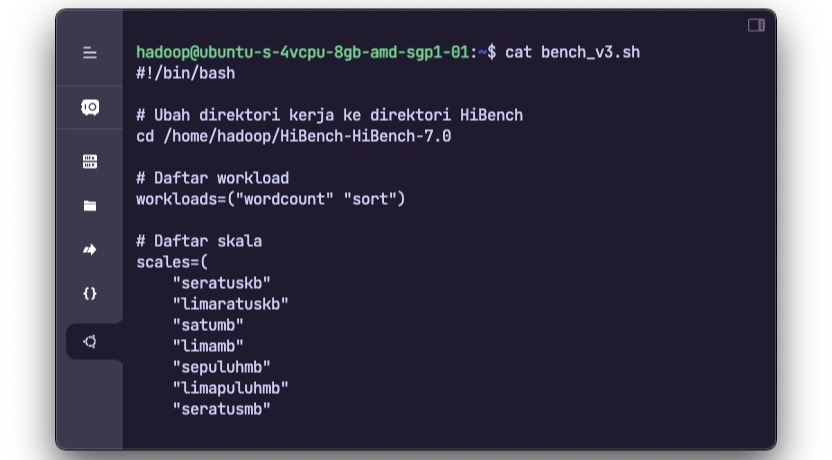
\includegraphics[width=0.75\textwidth]{figures/ch02/contoh-bash}
    \caption{Contoh Shell Script yang Digunakan pada Penelitian}
    \label{fig:contoh-bash}
\end{figure}

Gambar \ref{fig:contoh-bash} menampilkan sebuah contoh potongan \textit{shell script} yang digunakan dalam penelitian ini. Berikut adalah penjelasan lebih rinci mengenai skrip tersebut,
\begin{enumerate}
    \item \textbf{Baris 1:} Mendefinisikan interpreter Bash untuk menjalankan skrip.
    \item \textbf{Baris 3-4: } Mengubah direktori kerja ke direktori HiBench.
    \item \textbf{Baris 6-7: } Mendefinisikan daftar \textit{(list)} \textit{workLoads} berisi macam-macam beban kerja, yaitu \textit{wordcount} dan \textit{sort}.
    \item \textbf{Baris 9-15: } Mendefinisikan daftar \textit{scales} berisi skala input data.
\end{enumerate}

\section{\textit{CPU Bound} dan \textit{I/O Bound}}

Terdapat dua jenis beban kerja pada pemrosesan data berdasarkan karakteristik dan kebutuhan sumber daya yang berbeda, yaitu \textit{CPU-bound} dan \textit{I/O-bound}. Proses \textit{CPU-bound} (Gambar \ref{fig:cpu-bound} atas) sangat bergantung pada kemampuan pemrosesan data oleh \textit{Central Processing Unit} (CPU). Proses ini menghabiskan sebagian besar waktunya dalam menjalankan instruksi CPU dan jarang berinteraksi dengan sistem I/O (Input/Output). Sebaliknya, proses \textit{I/O-bound} (Gambar \ref{fig:cpu-bound} bawah) lebih banyak menghabiskan waktu dalam menunggu operasi I/O, seperti akses disk, jaringan, atau komunikasi peripheral. CPU dalam proses ini mungkin hanya digunakan sesaat untuk memproses data yang baru saja diperoleh dari I/O. 

Proses \textit{CPU-bound} memiliki interval waktu yang panjang untuk menjalankan instruksi CPU, dan jarang melakukan operasi I/O, yang dikenal sebagai \textit{CPU bursts} yang panjang dan jarang. Sementara itu, proses \textit{I/O-bound} memiliki interval waktu yang pendek untuk menjalankan instruksi CPU, dan sering melakukan operasi I/O, sehingga memiliki \textit{CPU bursts} yang pendek dan sering. 

\begin{figure}[h!]
    \centering
    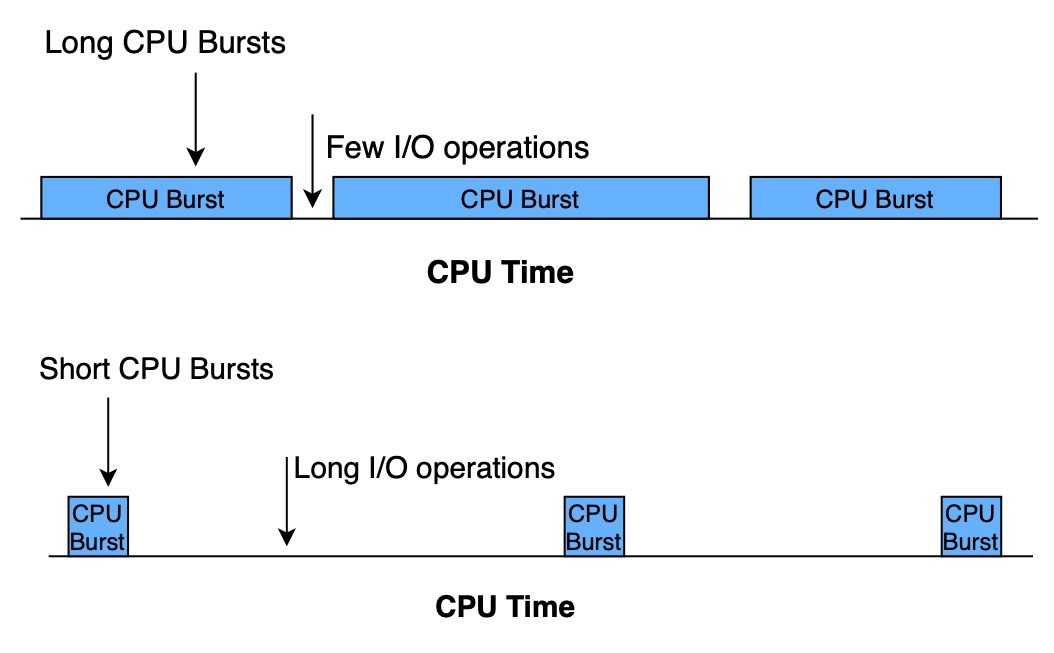
\includegraphics[width=0.8\textwidth]{figures/ch02/cpu-io-bound.jpg}
    \caption{\textit{CPU-I/O Bound} \cite{baeldungGuideCpuBoundBound2021}}
    \label{fig:cpu-bound}
\end{figure}


\section{MapReduce}
MapReduce adalah model pemrograman dan implementasi teknik pemrosesan data berukuran besar yang pertama kali dipopulerkan oleh Google pada tahun 2004\cite{kaliaAnalysisHadoopMapReduce2021}. MapReduce menawarkan pemrosesan data yang dapat diandalkan serta \textit{fault-tolerant manner} (tahan terhadap kesalahan).  MapReduce berjalan secara paralel dan berada pada lingkungan komputasi terdistribusi \cite{cTaskFailureResilience2020}. Model ini mengadopsi arsitektur tersentraliasi, yaitu satu \textit{node} berperan sebagai \textit{master} dan \textit{node} yang lain berperan sebagai \textit{workers} atau \textit{slave} \cite{herodotouHadoopPerformanceModels2011, bakratsasHadoopMapReducePerformance2018}. \textit{Master node} bertanggung jawab untuk melakukan penjadwalan kerja, dan \textit{slave node} berperan untuk menjalankan eksekusi kerja. 

\begin{figure}[h!]
    \centering
    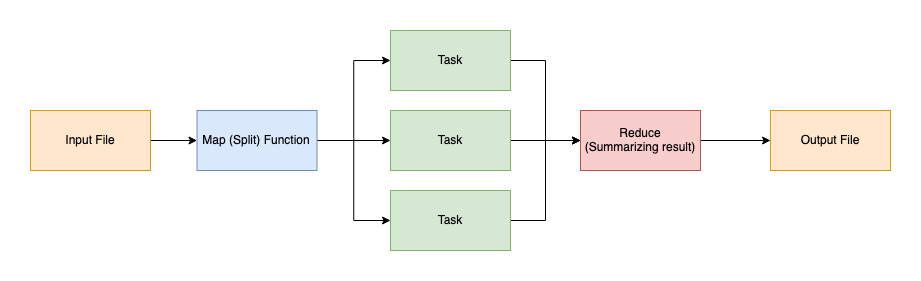
\includegraphics[width=1\textwidth]{figures/ch02/mapreduce-scheme.png}
    \caption{Cara Kerja MapReduce}
    \label{fig:mapreduce-flow}
\end{figure}

MapReduce terdiri dari fungsi \textit{Map} dan fungsi \textit{Reduce} \cite{gandomiHybSMRPHybridScheduling2019}. Kedua fungsi ini tersebar di seluruh \textit{slave node} yang terhubung dalam klaster dan berjalan secara paralel. Fungsi \textit{Map} berperan untuk membagi masalah besar menjadi masalah yang lebih kecil dan mendistribusikannya ke \textit{slave node}. Hasil pemrosesan dari \textit{slave node} akan dikumpulkan oleh \textit{master node} melalui fungsi \textit{Reduce}. Sesuai dengan Gambar \ref{fig:mapreduce-flow}, hasil dari proses \textit{Reduce} yang akan dikirimkan sebagai hasil akhir proses MapReduce.  

\subsection{Apache Hadoop}
Apache Hadoop adalah perangkat lunak sumber terbuka yang ditulis dengan bahasa pemrograman Java untuk pemrosesan dan penyimpanan data menggunakan komputasi terdistribusi \cite{ApacheHadoop}. Hadoop dapat diinstalasi pada satu \textit{node} komputer, atau ratusan \textit{node} komputer yang digabungkan dalam sebuah klaster \cite{maneasEvolutionHadoopDistributed2018}. Berkaitan dengan pemrosesan data, Hadoop mengimplementasikan model MapReduce untuk pemrosesan data secara paralel dan cepat. Selain itu, Hadoop menyediakan sistem penyimpanan data terdistribusi yang dikenal sebagai Hadoop Distributed File System (HDFS) untuk akses data, pemrosesan, dan komputasi \cite{dabasAnalysisCommentsYoutube2019}. Arsitektur Hadoop secara umum dapat dilihat pada Gambar \ref{fig:hadoop-str}.

\begin{figure}[h!]
    \centering
    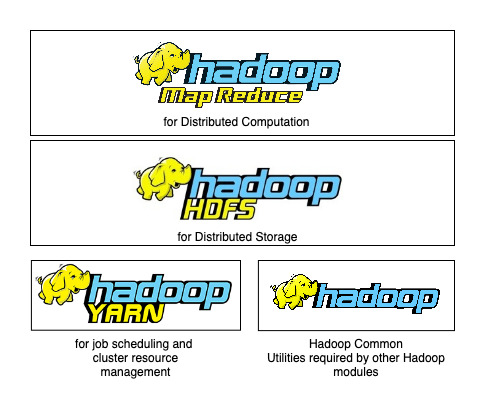
\includegraphics[width=0.6\textwidth]{figures/ch02/hadoop-str}
    \caption{Arsitektur Hadoop}
    \label{fig:hadoop-str}
\end{figure}

\subsection{Mode Kerja Hadoop}
Hadoop dapat dijalankan dalam tiga mode operasi yang berbeda yaitu \textit{standalone, pseudo-distributed}, dan \textit{fully distributed} \cite{johnDataLakeEnterprises2017}. Dalam \textit{standalone mode}, semua proses Hadoop berjalan pada satu node tunggal menggunakan sistem berkas lokal tanpa memerlukan konfigurasi kustom pada Hadoop seperti pada Gambar \ref{fig:hadoop-modes}. 

\begin{figure}[h!]
    \centering
    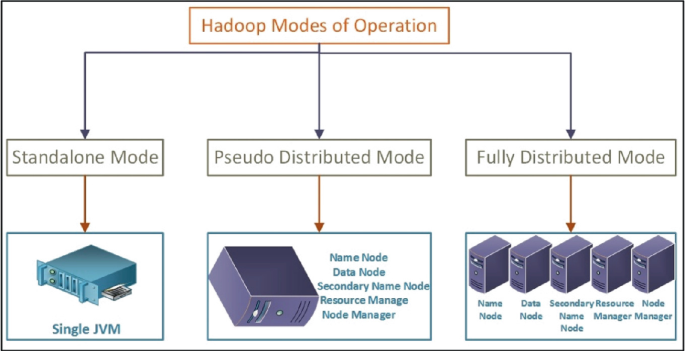
\includegraphics[width=0.9\textwidth]{figures/ch02/hadoop-modes}
    \caption{Mode Kerja Hadoop \cite{khataiImplementationTextMining2021}}
    \label{fig:hadoop-modes}
\end{figure}

\textit{Pseudo-distributed mode} menjalankan semua komponen Hadoop pada satu node tunggal tetapi menyimulasikan kluster dengan komunikasi antar proses melalui socket jaringan, sehingga memerlukan konfigurasi pada berkas \textit{core-site, mapred-site}, dan \textit{hdfs-site}. Sedangkan \textit{fully distributed mode} menyebarkan proses Hadoop ke beberapa node dalam kluster sebenarnya yang biasanya digunakan untuk tahap produksi. \textit{Fully distributed mode} mendukung skalabilitas, ketersediaan tinggi, dan keamanan dengan memerlukan instalasi Hadoop dan konfigurasi kluster pada setiap node.

\subsection{Hadoop Distributed File System (HDFS)}
\textit{Hadoop Distributed File System} adalah sistem file terdistribusi yang dikembangkan sebagai bagian dari Hadoop \cite{abhishekIntegratedHadoopCloud2017}. HDFS dirancang khusus untuk menyimpan data dalam jumlah besar dan memungkinkan pemrosesan data secara paralel. Beberapa fitur utama dari HDFS antara lain skalabilitas, toleransi kesalahan, \textit{streaming access}, dan cocok untuk aplikasi \textit{batch} seperti MapReduce.

\begin{figure}[h!]
    \centering
    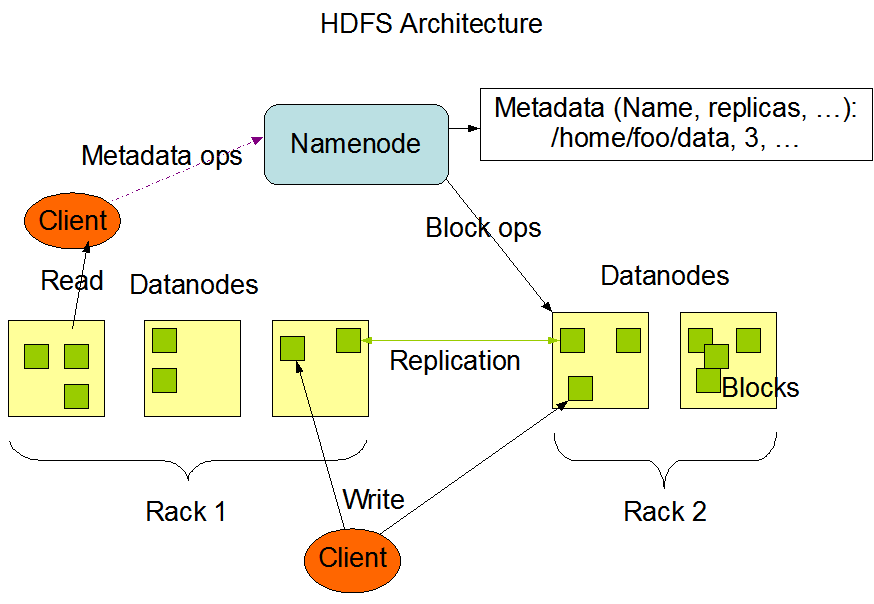
\includegraphics[width=0.8\textwidth]{figures/ch02/hdfsarchitecture}
    \caption{Arsitektur HDFS \cite{ApacheHadoopHDFS}}
    \label{fig:hdfs-arch}
\end{figure}

Secara struktur, HDFS terdiri dari NameNode sebagai \textit{node master} yang mengelola \textit{metadata} dan \textit{namespace}, serta DataNode sebagai \textit{node slave} yang bertugas menyimpan data sebenarnya dalam bentuk blok seperti pada Gambar \ref{fig:hdfs-arch}. Berkas di HDFS dipartisi menjadi satu atau lebih blok berukuran 64MB atau 128MB, kemudian didistribusikan dan disimpan di beberapa DataNode. Setiap blok direplikasi di DataNode yang berbeda untuk toleransi kesalahan. Replikasi blok di \textit{node/rack} yang berbeda juga meningkatkan ketersediaan HDFS.

Dengan desain terdistribusi, HDFS sangat populer digunakan bersama framework Hadoop untuk memproses \textit{big data} \cite{almansouriHadoopDistributedFile2019}. Namun, ketergantungan pada \textit{single} NameNode dan performa akses data acak yang kurang optimal menjadi kelemahan utama HDFS. Secara keseluruhan, HDFS telah terbukti menjadi pilihan matang untuk penyimpanan data massal secara terdistribusi.

\subsection{Hadoop YARN}
\textit{Hadoop YARN} (\textit{Yet Another Resource Negotiator}) adalah manajer sumber daya dan sistem penjadwalan untuk kluster Hadoop. Komponen ini diperkenalkan dalam Hadoop 2.x sebagai evolusi dari Hadoop MapReduce 1.x, yang mengintegrasikan manajemen sumber daya dan pemrosesan data dalam satu sistem. YARN memungkinkan kluster untuk menjalankan berbagai aplikasi secara bersamaan dengan efisiensi yang lebih baik.  YARN memisahkan fungsi manajemen sumber daya dari mekanisme pemrosesan data, yang sebelumnya keduanya tertanam dalam MapReduce. Dengan demikian, YARN dapat mendukung berbagai paradigma pemrosesan data di atas Hadoop, selain MapReduce, seperti \textit{real-time processing} dan \textit{graph processing}.

\begin{figure}[h!]
    \centering
    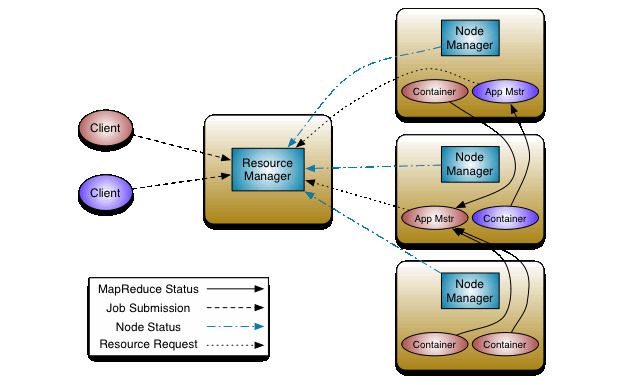
\includegraphics[width=0.8\textwidth]{figures/ch02/yarn-arch}
    \caption{Arsitektur YARN \cite{ApacheHadoopApache}}
    \label{fig:yarn_arch}
\end{figure}

Struktur utama YARN terdiri dari ResourceManager yang bertugas mengkoordinasikan alokasi sumber daya di seluruh kluster, dan NodeManager yang berjalan di setiap \textit{node} untuk mengawasi penggunaan sumber daya dan mengelola \textit{container} tempat aplikasi dijalankan. \textit{ApplicationMaster} adalah komponen khusus untuk setiap aplikasi yang bertanggung jawab untuk negosiasi sumber daya dengan ResourceManager dan bekerja dengan NodeManager untuk menjalankan dan memantau \textit{tasks} seperti pada Gambar \ref{fig:yarn_arch}.

\section{Apache Spark}
Apache Spark diperkenalkan oleh Apache Software Foundation sebagai \textit{framework} pemrosesan data paralel \textit{open-source} yang dirancang untuk mempercepat pemrosesan \textit{big data} dibandingkan dengan  Hadoop MapReduce \cite{ApacheSparkUnified}. Meskipun sama-sama menggunakan model pemrosesan MapReduce, Spark bukanlah hasil modifikasi dari Hadoop MapReduce\cite{KOMPARASIKECEPATANHADOOP}. Hal ini dikarenakan Spark menggunakan teknologi tersendiri yaitu \textit{Resilient Distributed Datasets} (RDDs) yang memungkinkan Spark memproses data secara \textit{in-memory} sehingga lebih cepat. Selain itu, Spark memiliki klaster pengolahan data tersendiri sehingga dapat berjalan independen tanpa Hadoop. Dengan performa tinggi serta dukungan untuk pemrosesan data secara interaktif, Spark banyak digunakan untuk pemrosesan data skala besar. Komponen yang terdapat pada Spark dapat dilihat pada Gambar \ref{fig:spark-component}

\begin{figure}[h]
    \centering
    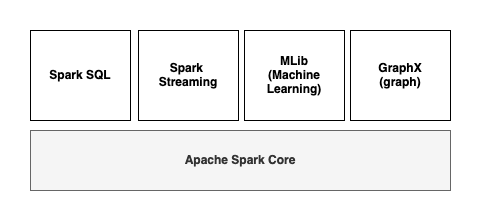
\includegraphics[width=0.6\textwidth]{figures/ch02/spark-contain}
    \caption{Komponen Spark}
    \label{fig:spark-component}
\end{figure}

\subsection{Arsitektur Spark}

Arsitektur Spark dirancang untuk pemrosesan data terdistribusi yang efisien dan cepat seperti pada Gambar \ref{fig:spark-arch}. Komponen utamanya meliputi \textit{Spark Driver, Cluster Manager}, dan \textit{Spark Executor}. \textit{Spark Driver} berperan sebagai otak operasi, bertanggung jawab untuk mengonversi program pengguna menjadi tugas-tugas, menjadwalkan tugas pada \textit{executor}, dan mengelola keseluruhan alur kerja. \textit{Cluster Manager}, yang dapat berupa YARN, Mesos, atau mode \textit{standalone} Spark, menangani alokasi sumber daya dan peluncuran \textit{executor} pada \textit{node-node cluster}. \textit{Spark Executor}, yang berjalan pada \textit{node-node cluster}, menjalankan tugas-tugas pemrosesan data yang diberikan oleh \textit{driver} dan menyediakan penyimpanan dalam memori untuk data yang di-\textit{cache}. Interaksi antara komponen-komponen ini memungkinkan pemrosesan data paralel yang cepat dan toleransi kesalahan yang tinggi. Arsitektur Spark yang fleksibel mendukung berbagai bahasa pemrograman dan sistem penyimpanan data, menjadikannya solusi ideal untuk berbagai kasus penggunaan data besar.

\begin{figure}[h]
    \centering
    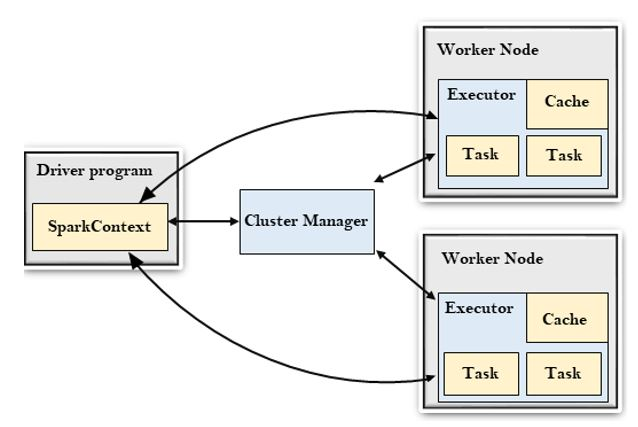
\includegraphics[width=0.6\textwidth]{figures/ch02/spark-arch.jpeg}
    \caption{Arsitektur Spark}
    \label{fig:spark-arch}
\end{figure}

\subsection{Integrasi Hadoop dan Spark}
Integrasi Spark dengan Hadoop dapat dilakukan melalui tiga metode berbeda seperti pada Gambar \ref{fig:spark-x-hadoop}  \cite{ApacheSparkIntroduction}. Pertama, metode \textit{Standalone} mengharuskan Spark menempati tempat di atas HDFS (\textit{Hadoop Distributed File System}). Dalam skenario ini, Spark dan MapReduce berjalan berdampingan untuk menangani semua pekerjaan Spark pada kluster. Kedua, metode Hadoop Yarn memungkinkan Spark berjalan pada Yarn tanpa memerlukan instalasi sebelumnya atau akses \textit{root}. Hal ini memfasilitasi integrasi Spark ke dalam ekosistem Hadoop, atau memungkinkan komponen lain berjalan di atas integrasi Hadoop dan Spark. Terakhir, metode \textit{Spark in MapReduce} (SIMR). Dengan SIMR, pengguna dapat memulai Spark dan menggunakan \textit{shell}-nya tanpa memerlukan akses administratif. 

\begin{figure}[h!]
    \centering
    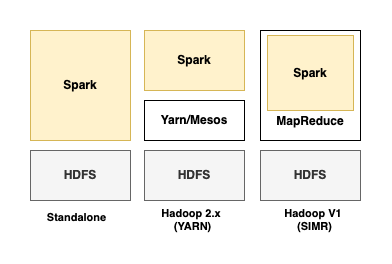
\includegraphics[width=0.7\textwidth]{figures/ch02/sparkxhadoop}
    \caption{Integrasi Spark dan Hadoop}
    \label{fig:spark-x-hadoop}
\end{figure}

%\section{\textit{Data Sharing} pada MapReduce dan Spark}
\subsection{Keterbatasan \textit{Data Sharing} pada MapReduce}

MapReduce, sebagai kerangka kerja pemrosesan data terdistribusi, mengandalkan sistem penyimpanan eksternal yang stabil, seperti HDFS, untuk berbagi data antar tugas (\textit{job}). Hal ini mengakibatkan inefisiensi karena beberapa alasan, yaitu:

\begin{enumerate}
    \item \textbf{Replikasi Data:} Data perlu direplikasi ke beberapa node untuk toleransi kesalahan dan paralelisme. Replikasi ini memakan waktu dan bandwidth jaringan.
    \item \textbf{Serialisasi/Deserialisasi:} Data perlu diubah formatnya (serialisasi) sebelum dikirim melalui jaringan dan diubah kembali (deserialisasi) di simpul tujuan. Proses ini menambah beban komputasi.
    \item \textbf{\textit{Disk} I/O:} Akses data dari dan ke disk cenderung lambat dibandingkan dengan akses memori. Pada MapReduce, setiap operasi baca-tulis data melibatkan interaksi dengan \textit{disk}, yang memperlambat performa.
\end{enumerate}

Keterbatasan ini terlihat jelas pada aplikasi yang membutuhkan operasi iteratif, di mana hasil antara dari satu tugas perlu digunakan kembali oleh tugas berikutnya. Pada MapReduce, setiap iterasi memerlukan pembacaan dan penulisan data ke HDFS, seperti yang diilustrasikan pada Gambar \ref{fig:iterative_operations_on_mapreduce}. Akibatnya, aplikasi iteratif pada MapReduce cenderung lambat dan tidak efisien.

\begin{figure}[h]
    \centering
    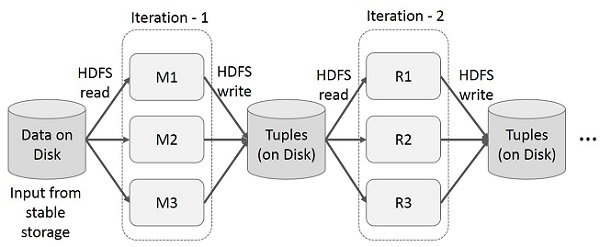
\includegraphics[width=1\textwidth]{figures/ch02/iterative_operations_on_mapreduce}
    \caption{\textit{Data Sharing} pada MapReduce \cite{ApacheSparkRDD}}
    \label{fig:iterative_operations_on_mapreduce}
\end{figure}

\subsection{Solusi \textit{Data Sharing} dengan Spark RDD}

Spark mengatasi keterbatasan MapReduce dengan memperkenalkan RDD, yaitu koleksi data terdistribusi yang disimpan dalam memori. RDD bersifat \textit{immutable}, artinya data tidak dapat diubah setelah dibuat, dan \textit{fault-tolerant}, artinya data dapat dipulihkan jika terjadi kegagalan node.

Dengan menyimpan data dalam memori, RDD memungkinkan akses data yang jauh lebih cepat dibandingkan dengan akses disk pada MapReduce. Selain itu, RDD mendukung \textit{lazy evaluation}, di mana operasi pada RDD tidak dieksekusi langsung, melainkan disimpan sebagai \textit{lineage} atau urutan operasi yang perlu dilakukan. Hal ini memungkinkan Spark untuk mengoptimalkan eksekusi tugas dan mengurangi overhead komputasi.

Pada aplikasi iteratif, RDD dapat menyimpan hasil antara dalam memori dan membagikannya antar tugas tanpa perlu mengakses disk, seperti yang ditunjukkan pada Gambar \ref{fig:iterative_operations_on_spark_rdd}. Dengan demikian, Spark RDD memungkinkan eksekusi aplikasi iteratif yang jauh lebih cepat dan efisien dibandingkan dengan MapReduce.

\begin{figure}[h]
    \centering
    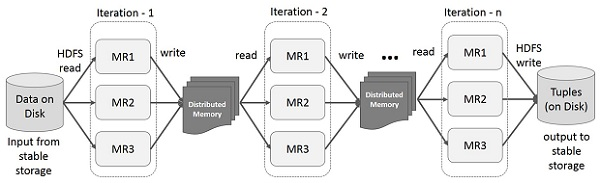
\includegraphics[width=1\textwidth]{figures/ch02/iterative_operations_on_spark_rdd}
    \caption{\textit{Data Sharing} pada RDD \cite{ApacheSparkRDD}}
    \label{fig:iterative_operations_on_spark_rdd}
\end{figure}

\section{HiBench}
HiBench memudahkan dalam eksekusi pengukuran berbagai beban kerja karena HiBench sudah membungkus sekumpulan perintah dalam bentuk \textit{shell script}\cite{samadiPerformanceComparisonHadoop2018}. Pengguna hanya perlu menjalankan perintah untuk HiBench melakukan persiapan data. Selanjutnya, pengguna bisa langsung melakukan pengukuran beban kerja. Hasilnya dapat terlihat langsung pada laporan HiBench. Secara umum, alur kerja HiBench terlihat seperti pada Gambar \ref{fig:hibench-process-flow}.

\begin{figure}[h]
    \centering
    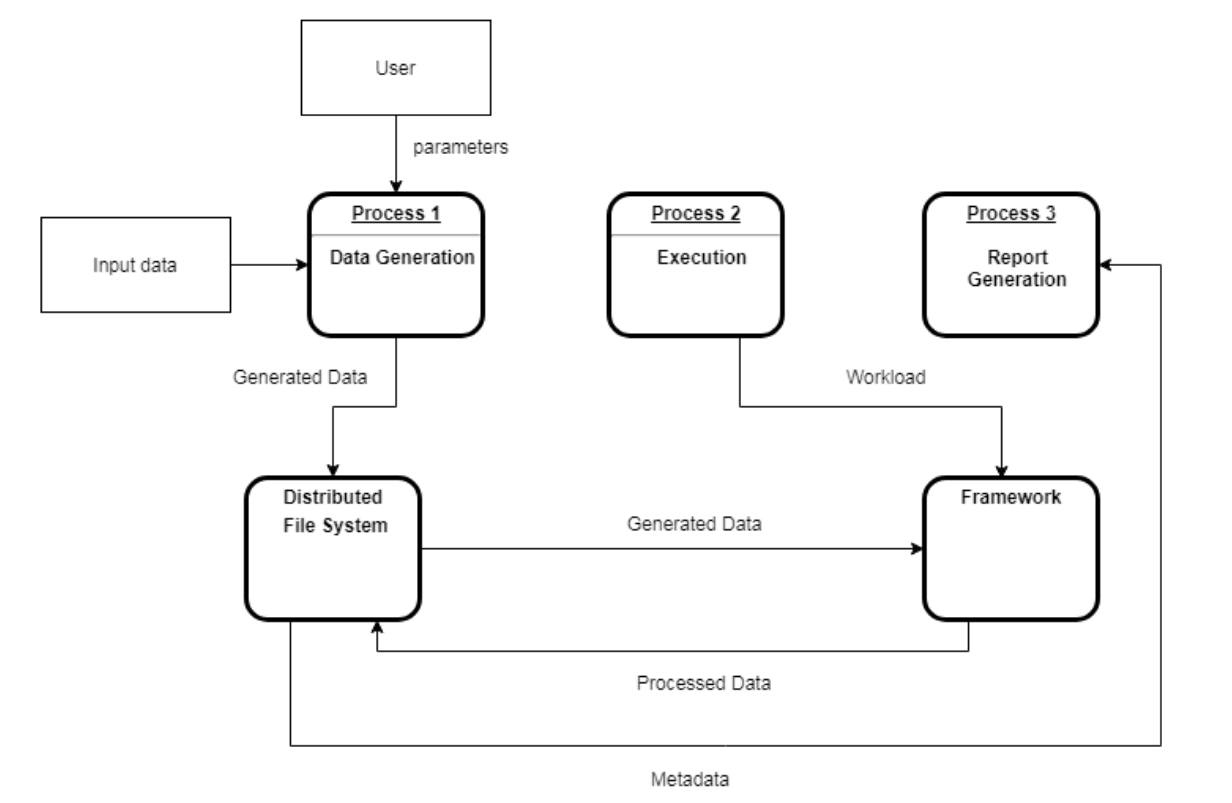
\includegraphics[width=1\textwidth]{figures/ch02/hibench-flow}
    \caption{Proses yang Terjadi di HiBench \cite{barosenAnalysisComparisonInterfacing2018}}
    \label{fig:hibench-process-flow}
\end{figure}

HiBench terdiri dari 3 proses utama. Proses pertama, pengguna melakukan konfigurasi parameter \textit{Data Generation}. Selanjutnya, \textit{Data Generation} akan melakukan pembentukan data yang nantinya akan disimpan pada \textit{Distributed File System} (DFS). Data ini yang akan digunakan pada proses selanjutnya. Proses kedua adalah proses eksekusi. Pengguna akan memicu salah satu beban kerja pada HiBench. Selanjutnya, HiBench akan memberi perintah kepada perangkat lunak (Hadoop/Spark) untuk menjalankan beban kerja tersebut. Setiap melakukan pengukuran, data yang digunakan adalah data dari \textit{Distributed File System} yang sebelumnya sudah dibentuk. Hasil dari eksekusi ini akan disimpan kembali di DFS. Proses terakhir adalah proses pembentukan laporan. Hasil dari proses sebelumnya akan diambil serta akan dibuatkan laporan secara otomatis.
Dalam laporan otomatis yang diberikan oleh HiBench, terdapat beberapa metriks yang tersedia, meliputi \textit{Execution Time} dan \textit{Throughput}. \textit{Execution Time} memiliki makna seberapa lama suatu kejadian berlangsung. Waktu yang dihitung adalah waktu diantara waktu awal dan waktu terakhir kejadian. Selanjutnya, \textit{Throughput} menghitung berapa banyak unit informasi yang dapat diproses oleh sistem dalam waktu tertentu. Metriks ini dinyatakan dalam \textit{byte}/detik.


\subsection{Beban Kerja \textit{Micro Benchmark} dan Sumber Data}
HiBench versi 7.1 memiliki 29 beban kerja (\textit{workload}) yang dapat diuji \cite{IntelbigdataHiBench2023}. Beban kerja ini dikategorikan menjadi 7 kategori, yaitu \textit{micro, ml (machine learning), sql, graph, websearch and streaming}. Tabel \ref{table:workload-list-hibench} menunjukkan macam-macam beban kerja yang dapat diuji. \textit{Workload name} mengindikasikan algoritma utama atau operasi apa yang dilakukan. \textit{Workload type} merepresentasikan kategori dari beban kerja. \textit{Operation types} menunjukkan klasifikasi jenis operasi yang dilakukan. \textit{Workload Submission Policy} berguna untuk mengetahui bagaimana cara pengguna untuk mengatur atau mengonfigurasikan beban kerja.

\begin{table}[h]
  \centering
  \caption{Beban Kerja pada HiBench \cite{barosenAnalysisComparisonInterfacing2018}}
  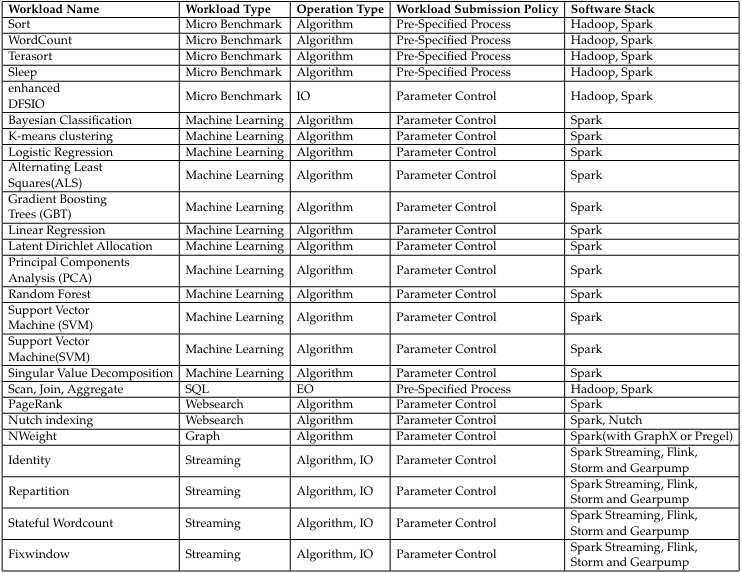
\includegraphics[width=1\textwidth]{figures/ch02/workload-hibench}
  \label{table:workload-list-hibench}
\end{table}

Beban kerja \textit{micro benchmarks} merupakan kategori khusus yang dirancang untuk menguji kemampuan \textit{raw processing power} \cite{barosenAnalysisComparisonInterfacing2018}. Dalam kategori ini, terdapat dua beban kerja populer, yaitu \textit{Sort}, dan \textit{Word Count} \cite{huangHiBenchBenchmarkSuitea}. Beban kerja \textit{Sort} dan \textit{Word Count} merepresentasikan pekerjaan MapReduce \cite{deanMapReduceSimplifiedData2004}. Beban kerja \textit{Sort} akan mengurutkan setiap kata dalam berkas input. Beban kerja \textit{Word Count} akan melakukan tugas pemetaan (\textit{map task}) dan mengeluarkan output (kata, 1) untuk setiap kata dalam inputnya.  Data masukan untuk beban kerja \textit{Sort} dan \textit{Word Count} dihasilkan menggunakan program RandomTextWriter yang nantinya akan dibuat melalui proses \textit{Data Generation}. 

\subsection{\textit{Data Generation} pada \textit{Word Count} dan \textit{Sort}}
\textit{Data generation} merupakan tahapan krusial dalam benchmark menggunakan HiBench, khususnya untuk beban kerja \textit{Word Count} dan \textit{Sort}. Tahapan ini bertanggung jawab untuk membentuk data acak yang akan diproses oleh kedua beban kerja tersebut. Tujuannya adalah untuk menyimulasikan skenario nyata dengan input data yang bervolume besar dan beragam.

Pada HiBench, skrip \textit{prepare.sh} seperti pada Algoritma \ref{algo:data-gen} berperan penting dalam menyiapkan data untuk beban kerja. Skrip ini mengeksekusi program RandomTextWriter yang terdapat dalam paket Hadoop. RandomTextWriter menghasilkan sekumpulan data acak yang terdiri dari kata-kata yang diambil dari daftar kata yang telah ditentukan. Jumlah data yang dihasilkan, jumlah \textit{map}, dan jumlah \textit{reduce} dapat dikonfigurasi melalui parameter-parameter yang diberikan kepada skrip \textit{prepare.sh}.

\begin{lstlisting}[language=bash, caption=Skrip yang Digunakan HiBench pada Tahap \textit{Data Generation}, label=algo:data-gen]
#!/bin/bash

current_dir=`dirname "$0"`
current_dir=`cd "$current_dir"; pwd`
root_dir=${current_dir}/../../../../../
workload_config=${root_dir}/conf/workloads/micro/sort.conf
. "${root_dir}/bin/functions/load_bench_config.sh"

enter_bench HadoopPrepareSort ${workload_config} ${current_dir}
show_bannar start

rmr_hdfs $INPUT_HDFS || true
START_TIME=`timestamp`

run_hadoop_job ${HADOOP_EXAMPLES_JAR} randomtextwriter \
    -D mapreduce.randomtextwriter.totalbytes=${DATASIZE} \
    -D mapreduce.randomtextwriter.bytespermap=$(( ${DATASIZE} / ${NUM_MAPS} )) \
    -D mapreduce.job.maps=${NUM_MAPS} \
    -D mapreduce.job.reduces=${NUM_REDS} \
    ${INPUT_HDFS}
END_TIME=`timestamp`
show_bannar finish
leave_bench
\end{lstlisting}

Dalam penerapannya, RandomTextWriter akan menghitung jumlah total \textit{map task} yang diperlukan berdasarkan konfigurasi dan status kluster Hadoop. Setiap \textit{map task} akan menulis data hingga mencapai jumlah bita yang telah dikonfigurasi, menghasilkan kata acak sesuai dengan panjang yang telah ditentukan. Kata acak tersebut berasal dari kamus (\textit{dictionary}) yang sebelumnya sudah didefinisikan seperti pada Gambar \ref{fig:contoh-data}.

Jika diberikan input yang pasti, misalnya 100 KB, RandomTextWriter memungkinkan menghasilkan keluaran dengan ukuran tersebut tanpa pemotongan kata, karena \textit{mapper} menghasilkan kata acak dalam satuan kata lengkap dan menghitung panjang kata-kata tersebut sebelum menulisnya.

\begin{figure}[h]
    \centering
    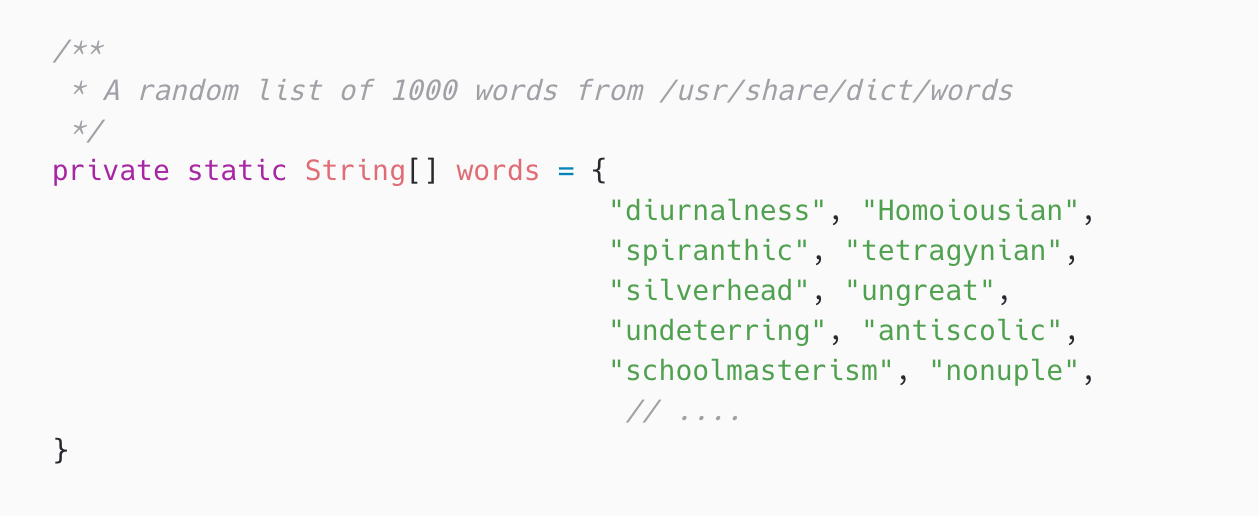
\includegraphics[width=0.85\textwidth]{figures/ch02/contoh-data}
    \caption{Contoh Kata pada \textit{Random Text Writer}}
    \label{fig:contoh-data}
\end{figure}


\subsection{Beban Kerja \textit{Word Count}}
\textit{Word Count} adalah algoritma sederhana untuk membaca berkas teks, dan menghitung jumlah kemunculan kata-kata pada file tersebut. Pada algoritma ini, inputnya berupa berkas teks dan outputnya berupa pasangan kata-kata dan jumlah kemunculannya. Beban kerja \textit{word count} akan menghasilkan data keluaran yang lebih kecil dari pada data input seperti pada Gambar \ref{fig:sample-wordcount}.
Karena itu, \textit{word count} memiliki sifat \textit{CPU Bound} yang nantinya akan ditandai dengan tingkat penggunaan CPU yang tinggi dan penggunaan I/O ringan. Selain itu, perilakunya diperkirakan akan tetap sama bahkan pada cluster yang lebih besar.

\begin{figure}[h]
    \centering
    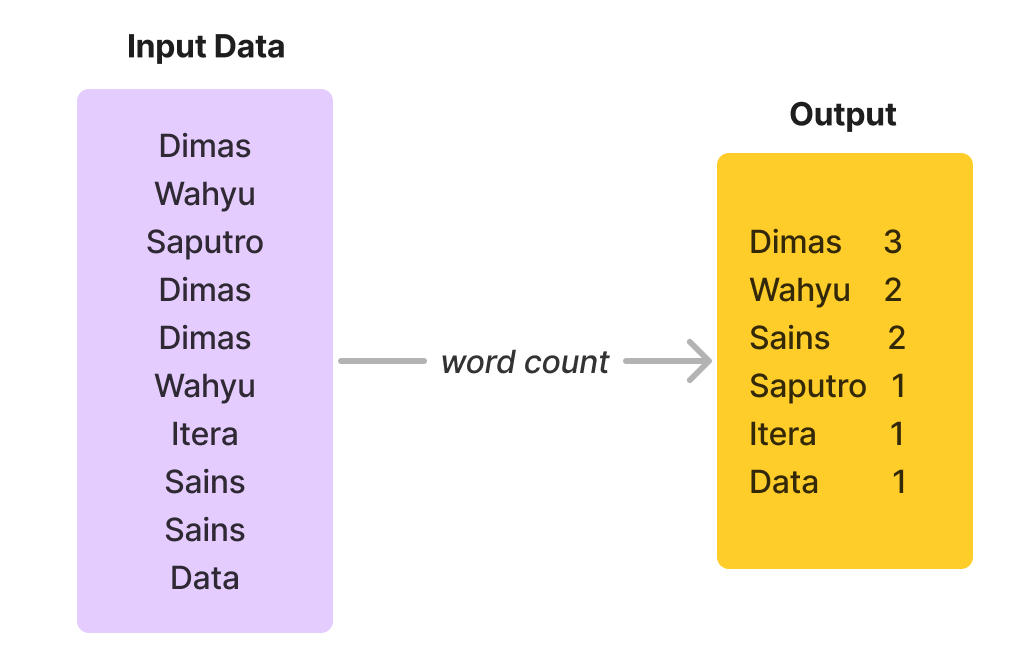
\includegraphics[width=0.7\textwidth]{figures/ch02/sample-wordcount.png}
    \caption{Contoh Input dan Output \textit{Word Count}}
    \label{fig:sample-wordcount}
\end{figure}

Implementasi MapReduce pada \textit{Word Count}\cite{KOMPARASIKECEPATANHADOOP} dapat dilihat pada Gambar \ref{fig:mapreduce-wordcount}. Pada proses MapReduce, data masukan akan melalui beberapa tahapan pemrosesan. Pertama, data akan dipecah menjadi bagian-bagian yang lebih kecil pada proses pemecahan data masukan (\textit{splitting}). Dalam kasus Hadoop MapReduce, data idealnya akan dipecah menjadi beberapa blok berukuran maksimal 128MB.

\begin{figure}[h]
    \centering
    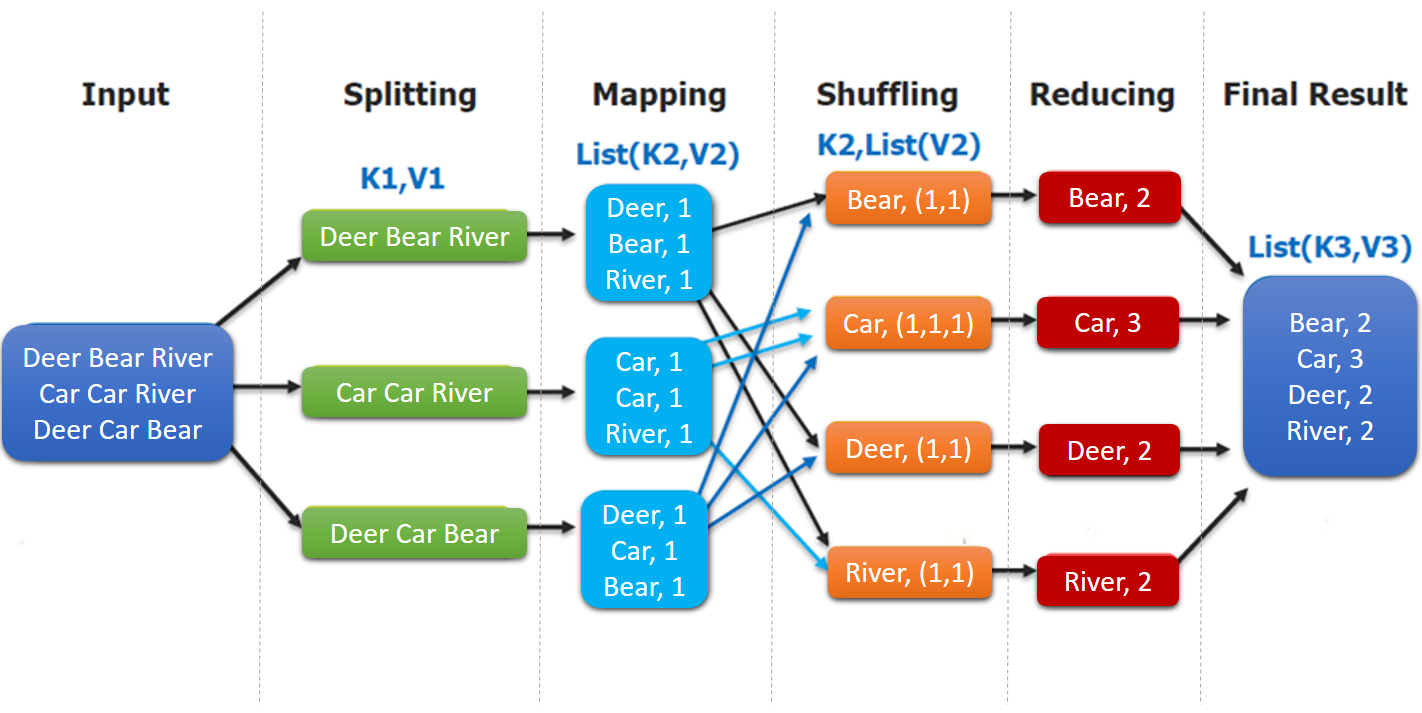
\includegraphics[width=0.85\textwidth]{figures/ch02/map-reduce-word-count-oreilly.png}
    \caption{Implementasi MapReduce pada Word Count \cite{MapReduceDistributedComputing}}
    \label{fig:mapreduce-wordcount}
\end{figure}

Kemudian, blok data tersebut akan diproses lebih lanjut pada tahap pemetaan (\textit{mapping}). Pemetaan merupakan salah satu tahapan terpenting dalam MapReduce. Pada tahap ini, blok data yang sudah dipecah akan diproses untuk menghasilkan pasangan kunci-nilai (\textit{key-value pairs}) sementara, seperti pada contoh kasus \textit{wordcount} yang menghasilkan pasangan kunci-nilai \textit{Dear:1, Bear:1, dan River:1}. Pemetaan dapat melibatkan satu atau beberapa mesin pekerja (\textit{worker}) yang memproses blok data secara paralel.

Selanjutnya adalah tahap pengocokan (\textit{shuffling}) di mana pasangan kunci-nilai hasil pemetaan yang tersebar di beberapa mesin akan dikumpulkan berdasarkan kesamaan kuncinya agar bisa diproses lebih lanjut. Misalnya semua pasangan dengan kunci \textit{Bear} dikumpulkan dalam satu mesin.

Pada tahap terakhir yaitu pengurangan (\textit{reducing}), dilakukan agregasi terhadap pasangan kunci-nilai dengan kunci yang sama untuk menghasilkan keluaran akhir. Seperti pada contoh kasus \textit{wordcount}, pasangan \textit{Bear:1} dan \textit{Bear:1} akan dijumlahkan menjadi \textit{Bear:2} oleh proses pengurangan.

\subsection{Beban Kerja \textit{Sort}}
\textit{Sort} adalah algoritma yang umum digunakan untuk mengurutkan data berdasarkan kriteria tertentu. Algoritma ini menerima data dalam bentuk acak sebagai input, dan menghasilkan data yang terurut sebagai output seperti pada Gambar \ref{fig:sample-sort}. Data input dan output memiliki ukuran yang sama, sehingga beban kerja sort tidak menghasilkan pengurangan data.
Kompleksitas algoritma \textit{sort} bervariasi, tetapi umumnya membutuhkan perbandingan dan pertukaran elemen data yang intensif. Oleh karena itu, beban kerja \textit{sort} cenderung bersifat I/O \textit{bound}, dengan pemanfaatan CPU yang rendah dan penggunaan I/O yang tinggi. 

\begin{figure}[h]
    \centering
    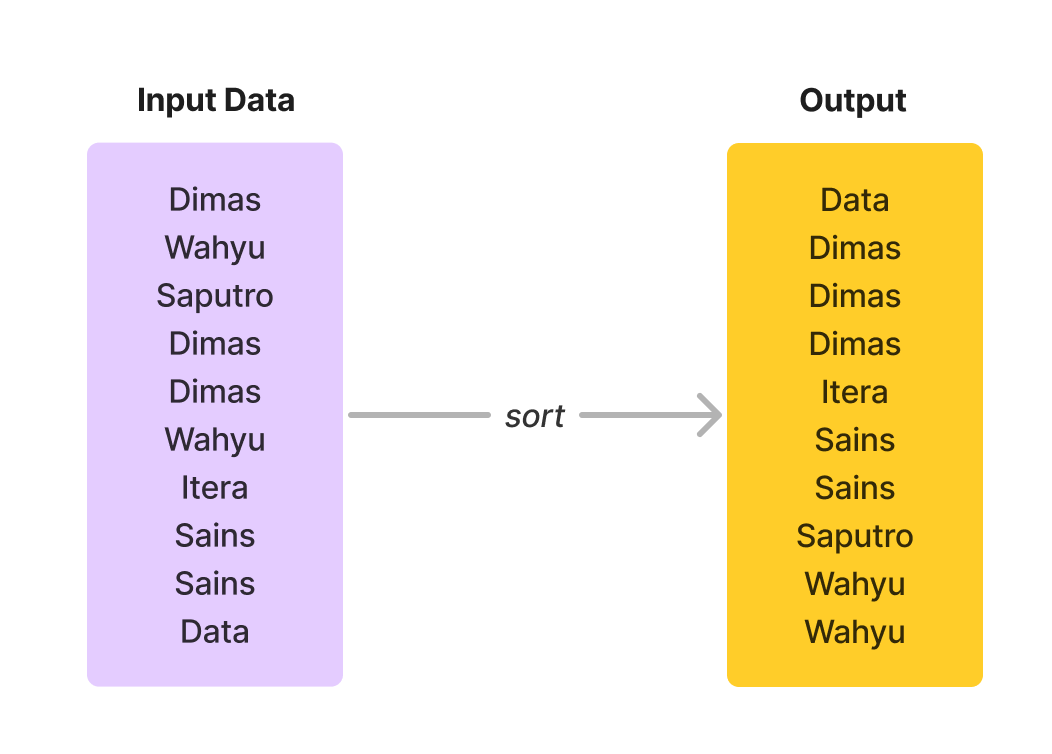
\includegraphics[width=0.7\textwidth]{figures/ch02/sample-sort}
    \caption{Contoh Input dan Output \textit{Sort}}
    \label{fig:sample-sort}
\end{figure}

%\subsection{Word Count - Hadoop}
%\begin{algorithm}[H]
%\caption{Word Count MapReduce}
%\SetKwInOut{Masukan}{Masukan}
%\SetKwInOut{Keluaran}{Keluaran}
%
%\Masukan{Berkas teks dengan setiap baris sebagai kalimat.}
%\Keluaran{Berkas sequence dengan setiap baris sebagai (kata, jumlah).}
%\BlankLine
%\textbf{Tahap Map:}\\
%\For{setiap baris $baris$ dalam teks masukan}{
%    $kata \gets tokenisasi(baris)$\;
%    \For{setiap kata $k$ dalam $kata$}{
%        Keluarkan($k$, 1)\;
%    }
%}
%\BlankLine
%\textbf{Tahap Combine (Opsional):}\\
%\For{setiap pasangan kunci-nilai ($k$, [$j_1, j_2, ..., j_n$])}{
%    $jumlah \gets \sum_{i=1}^{n} j_i$\;
%    Keluarkan($k$, $jumlah$)\;
%}
%\BlankLine
%\textbf{Tahap Reduce:}\\
%\For{setiap pasangan kunci-nilai ($k$, [$j_1, j_2, ..., j_n$])}{
%    $jumlah\_total \gets \sum_{i=1}^{n} j_i$\;
%    Keluarkan($k$, $jumlah\_total$)\;
%}
%\end{algorithm}
%
%\subsection{Word Count - Spark}
%\begin{algorithm}[H]
%\caption{Scala Word Count}
%\SetKwInOut{Masukan}{Masukan}
%\SetKwInOut{Keluaran}{Keluaran}
%
%\Masukan{Berkas teks pada HDFS dengan setiap baris sebagai kalimat.}
%\Keluaran{Berkas teks pada HDFS dengan setiap baris sebagai (kata, jumlah).}
%\BlankLine
%1. Inisialisasi SparkContext\;
%2. $data \gets$ Muat data teks dari HDFS\;
%3. $kata \gets$ Pisahkan setiap baris dalam $data$ menjadi kata-kata individual\;
%4. $pasangan \gets$ Ubah setiap kata menjadi pasangan (kata, 1)\;
%5. $jumlah \gets$ Jumlahkan nilai untuk setiap kata menggunakan `reduceByKey`\;
%6. Simpan $jumlah$ ke HDFS\;
%7. Hentikan SparkContext\;
%\end{algorithm}


%\subsection{Beban Kerja Sort}
%\blindtext

%\subsection{Sort - Hadoop}
%\begin{algorithm}[H]
%\caption{Sort Hadoop MapReduce}
%\SetKwInOut{Masukan}{Masukan}
%\SetKwInOut{Keluaran}{Keluaran}
%
%\Masukan{Data pada HDFS (format dapat ditentukan)}
%\Keluaran{Data terurut pada HDFS (format dapat ditentukan)}
%\BlankLine
%\textbf{Inisialisasi:}\\
%1. Inisialisasi konfigurasi dan JobClient\;
%2. Tentukan jumlah reducer berdasarkan konfigurasi dan kapasitas cluster\;
%3. Tentukan format input, format output, kelas kunci output, dan kelas nilai output (dapat ditentukan pengguna)\;
%4. Buat objek Job dan atur konfigurasi dasar (nama, jar, mapper, reducer, jumlah reducer, format input/output, kelas kunci/nilai output)\;
%5. Atur lokasi input dan output pada HDFS\;
%6. \If{pengguna meminta total-order sort}{
%    Lakukan sampling data input\;
%    Buat berkas partisi untuk total-order sort\;
%    Atur konfigurasi total-order sort pada job\;
%}
%\BlankLine
%\textbf{Tahap Map:}\\
%\For{setiap masukan (kunci, nilai)}{
%    Emit (keluarkan) pasangan (kunci, nilai)\;
%}
%\BlankLine
%\textbf{Tahap Reduce:}\\
%\For{setiap (kunci, [nilai1, nilai2, ...])}{
%    \For{setiap nilai $v$ dalam daftar nilai}{
%        Emit (keluarkan) pasangan (kunci, $v$)\;
%    }
%}
%\BlankLine
%\textbf{Eksekusi:}\\
%7. Cetak informasi job (node, lokasi input/output, jumlah reducer)\;
%8. Jalankan job dan tunggu hingga selesai\;
%9. Cetak waktu eksekusi job\;
%\end{algorithm}

%\subsection{Sort - Spark}
%\begin{algorithm}[H]
%\caption{Scala Sort}
%\SetKwInOut{Masukan}{Masukan}
%\SetKwInOut{Keluaran}{Keluaran}
%
%\Masukan{Berkas teks pada HDFS}
%\Keluaran{Berkas teks terurut pada HDFS}
%\BlankLine
%1. Inisialisasi SparkContext\;
%2. Tentukan jumlah partisi untuk pengurutan\;
%3. $data \gets$ Muat data teks dari HDFS dan ubah setiap baris menjadi pasangan (baris, 1)\;
%4. Buat objek HashPartitioner dengan jumlah partisi yang ditentukan\;
%5. $terurut \gets$ Urutkan $data$ berdasarkan kunci menggunakan `sortByKeyWithPartitioner` dengan HashPartitioner\;
%6. Ambil nilai dari setiap pasangan terurut (yaitu, hanya teks baris)\;
%7. Simpan data terurut $terurut$ ke HDFS\;
%8. Hentikan SparkContext\;
%\end{algorithm}

\section{Data Keluaran HiBench dan Dool}
Diagram pada Gambar \ref{fig:output-hibench-dool} mengilustrasikan data keluaran dari dua alat, yaitu HiBench dan Dool, yang digunakan untuk mengevaluasi kinerja sistem. HiBench berfokus pada pengukuran kinerja keseluruhan dari suatu beban kerja (\textit{benchmark}), sementara Dool memberikan pemantauan sistem yang terperinci secara \textit{real-time}.

\subsection{HiBench \textit{Report}}
HiBench menghasilkan laporan yang mencakup dua metrik utama, yaitu
\begin{enumerate}
	\item \textbf{Waktu Eksekusi (\textit{Execution Time})}: Waktu eksekusi suatu proses dapat dihitung dengan mengambil perbedaan antara waktu akhir dan waktu awal dari proses tersebut dalam format \textit{timestamp}. \textit{Timestamp} yang digunakan adalah dalam bentuk \textit{Unix time}, yaitu representasi waktu sebagai jumlah detik yang telah berlalu sejak 1 Januari 1970 UTC. Untuk mendapatkan waktu eksekusi, pertama-tama catat waktu awal proses menggunakan \textit{timestamp Unix}. Setelah proses selesai, catat waktu akhirnya dengan cara yang sama. Selanjutnya, kurangi waktu awal dari waktu akhir untuk memperoleh durasi eksekusi dalam satuan detik.
	\item \textbf{\textit{Throughput}}: Mengukur jumlah data yang diproses per satuan waktu, biasanya dalam bita (\textit{byte}) per detik. Metrik ini mencerminkan efisiensi sistem dalam menangani beban kerja. Ilustrasi \textit{Throughput} terlihat seperti pada Gambar \ref{fig:ilustrasi-throughput}
\end{enumerate}

\begin{figure}[h]
    \centering
    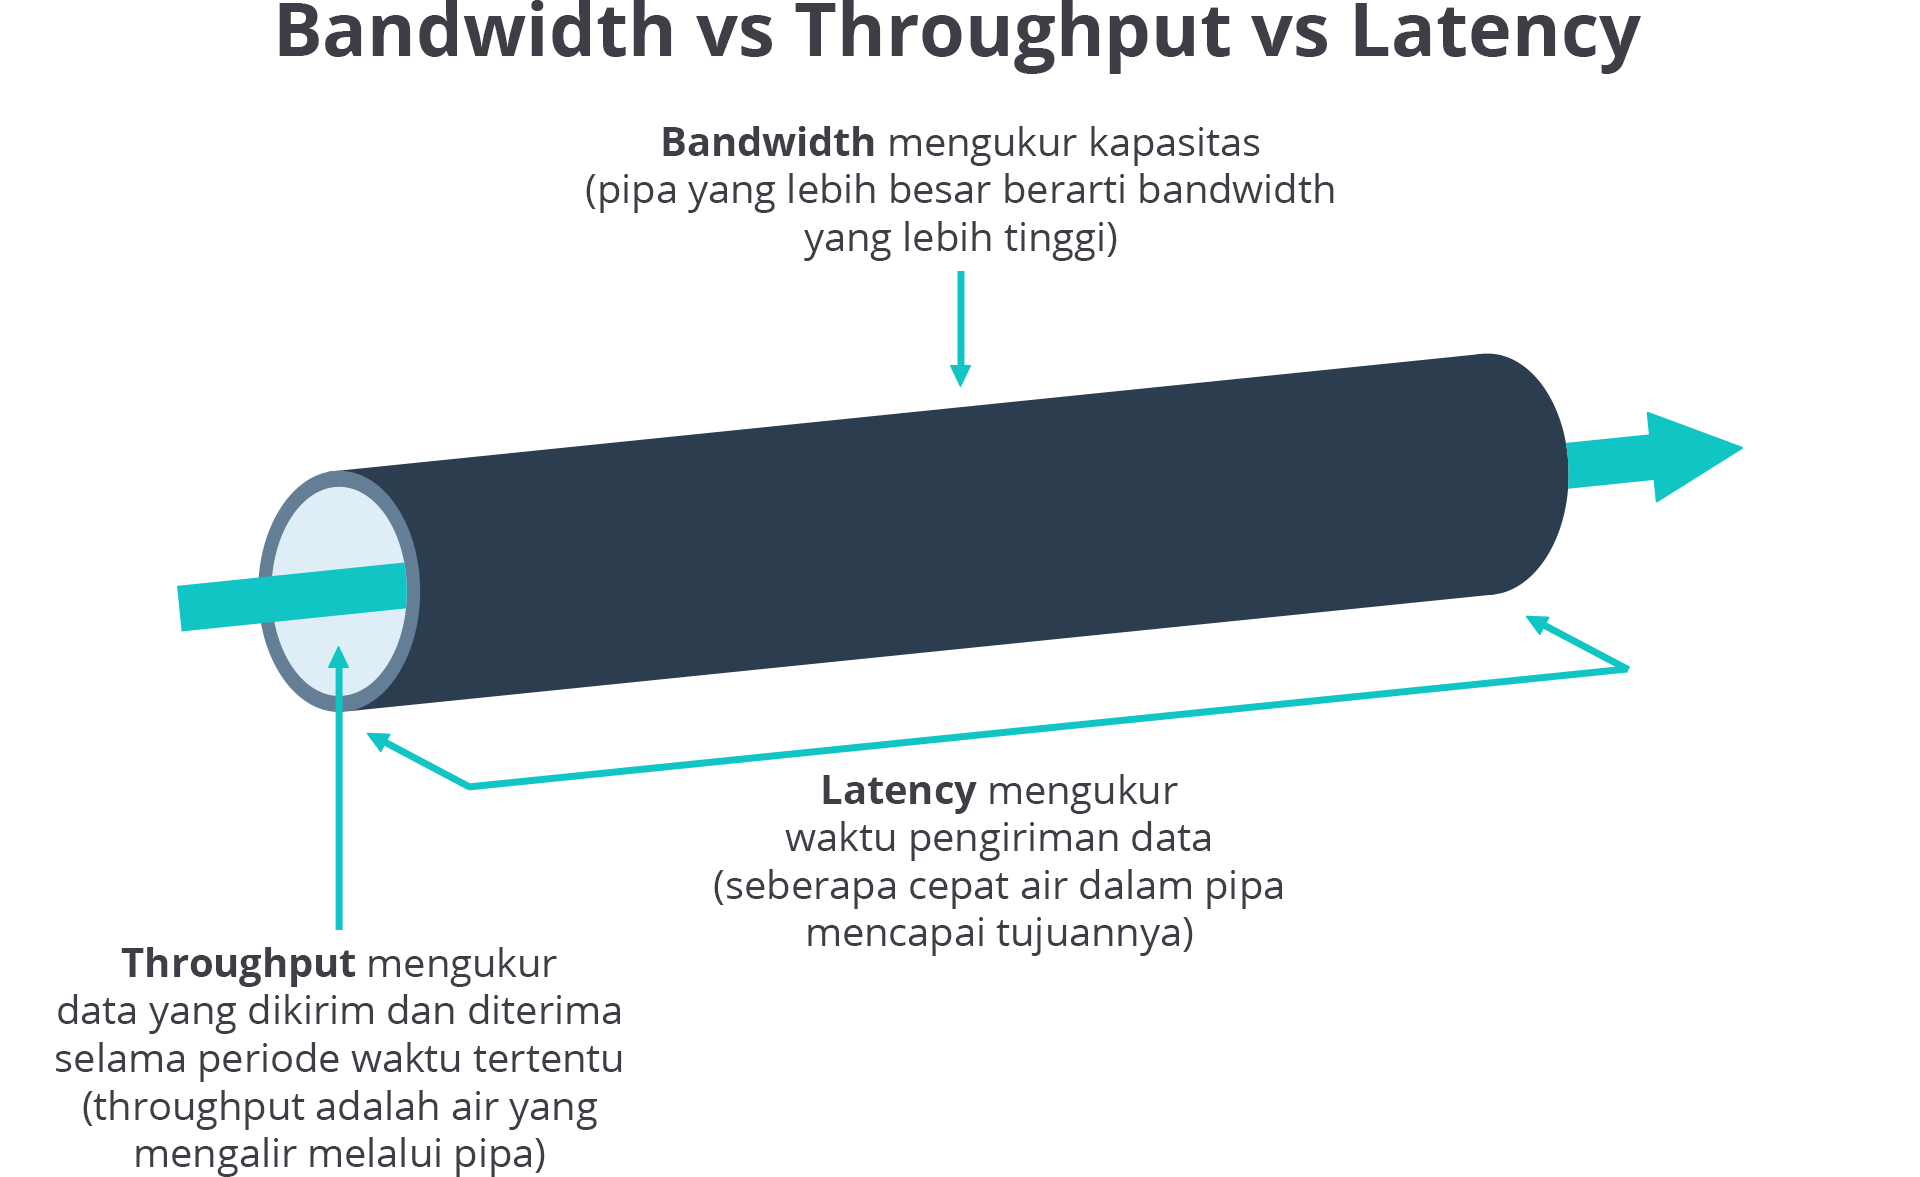
\includegraphics[width=0.7\textwidth]{figures/ch02/ilustrasi-lalu-lintas-jaringan.png}
    \caption{Ilustrasi \textit{Throughput} \cite{PenjelasanApaItu2023}}
    \label{fig:ilustrasi-throughput}
\end{figure}



\subsection{Dool: \textit{System Monitoring}}
Dool menyediakan pemantauan sistem yang mendetail dan diperbarui setiap detik. Data keluaran Dool meliputi berbagai aspek kinerja sistem, antara lain:
\begin{enumerate}
	\item \textbf{\textit{Time}}: \textit{Timestamp} yang menunjukkan waktu pengambilan data.
	\item \textbf{\textit{Date}}: Tanggal pengambilan 
	\item \textbf{\textit{Type}}: Jenis pengukuran yang dilakukan, misalnya CPU, memori, disk, atau jaringan. 
	\item \textbf{io/total}: Total aktivitas input/output (I/O) pada \textit{disk}, diukur dalam jumlah operasi I/O per 
	\item \textbf{\textit{total cpu usage}}: Persentase penggunaan CPU secara keseluruhan. 
		\begin{enumerate}
		\item \textbf{\textit{cpu/user}}: Persentase waktu CPU yang digunakan oleh proses-proses di ruang pengguna (\textit{user space}). Ini mencerminkan aktivitas dari aplikasi-aplikasi dan proses-proses yang dijalankan oleh pengguna.
		\item \textbf{\textit{cpu/wait}}: Persentase waktu CPU yang dihabiskan untuk menunggu operasi I/O selesai. Angka yang tinggi pada metrik ini bisa menunjukkan adanya \textit{bottleneck} pada disk atau jaringan yang menyebabkan CPU harus menunggu data tersedia.
		\end{enumerate}
	\item \textbf{\textit{disk/total}}: Total aktivitas \textit{disk}, mencakup baca dan tulis, diukur dalam bita per detik.
		\begin{enumerate}
		\item \textbf{\textit{disk/read}}: Jumlah data yang dibaca dari disk, diukur dalam bita per detik. Metrik ini penting untuk mengidentifikasi seberapa banyak beban pembacaan yang diterima oleh sistem penyimpanan.
		\item \textbf{\textit{disk/write}}: Jumlah data yang ditulis ke disk, diukur dalam bita per detik. Metrik ini menunjukkan seberapa banyak data yang sedang ditulis ke penyimpanan, yang bisa mempengaruhi kinerja sistem jika terlalu tinggi.
		\end{enumerate}
	\item \textbf{\textit{memory usage}}: Jumlah memori yang sedang digunakan oleh sistem.
	\item \textbf{net/total}: Total aktivitas jaringan, mencakup data yang dikirim dan diterima, diukur dalam bita per detik.
\end{enumerate}

Akhirnya, HiBench memberikan gambaran umum tentang efisiensi sistem dalam menangani beban kerja tertentu, sementara Dool memungkinkan kita untuk memantau berbagai komponen sistem secara\textit{ real-time} dan mengidentifikasi potensi \textit{bottleneck} atau masalah kinerja.

\begin{figure}[h]
    \centering
    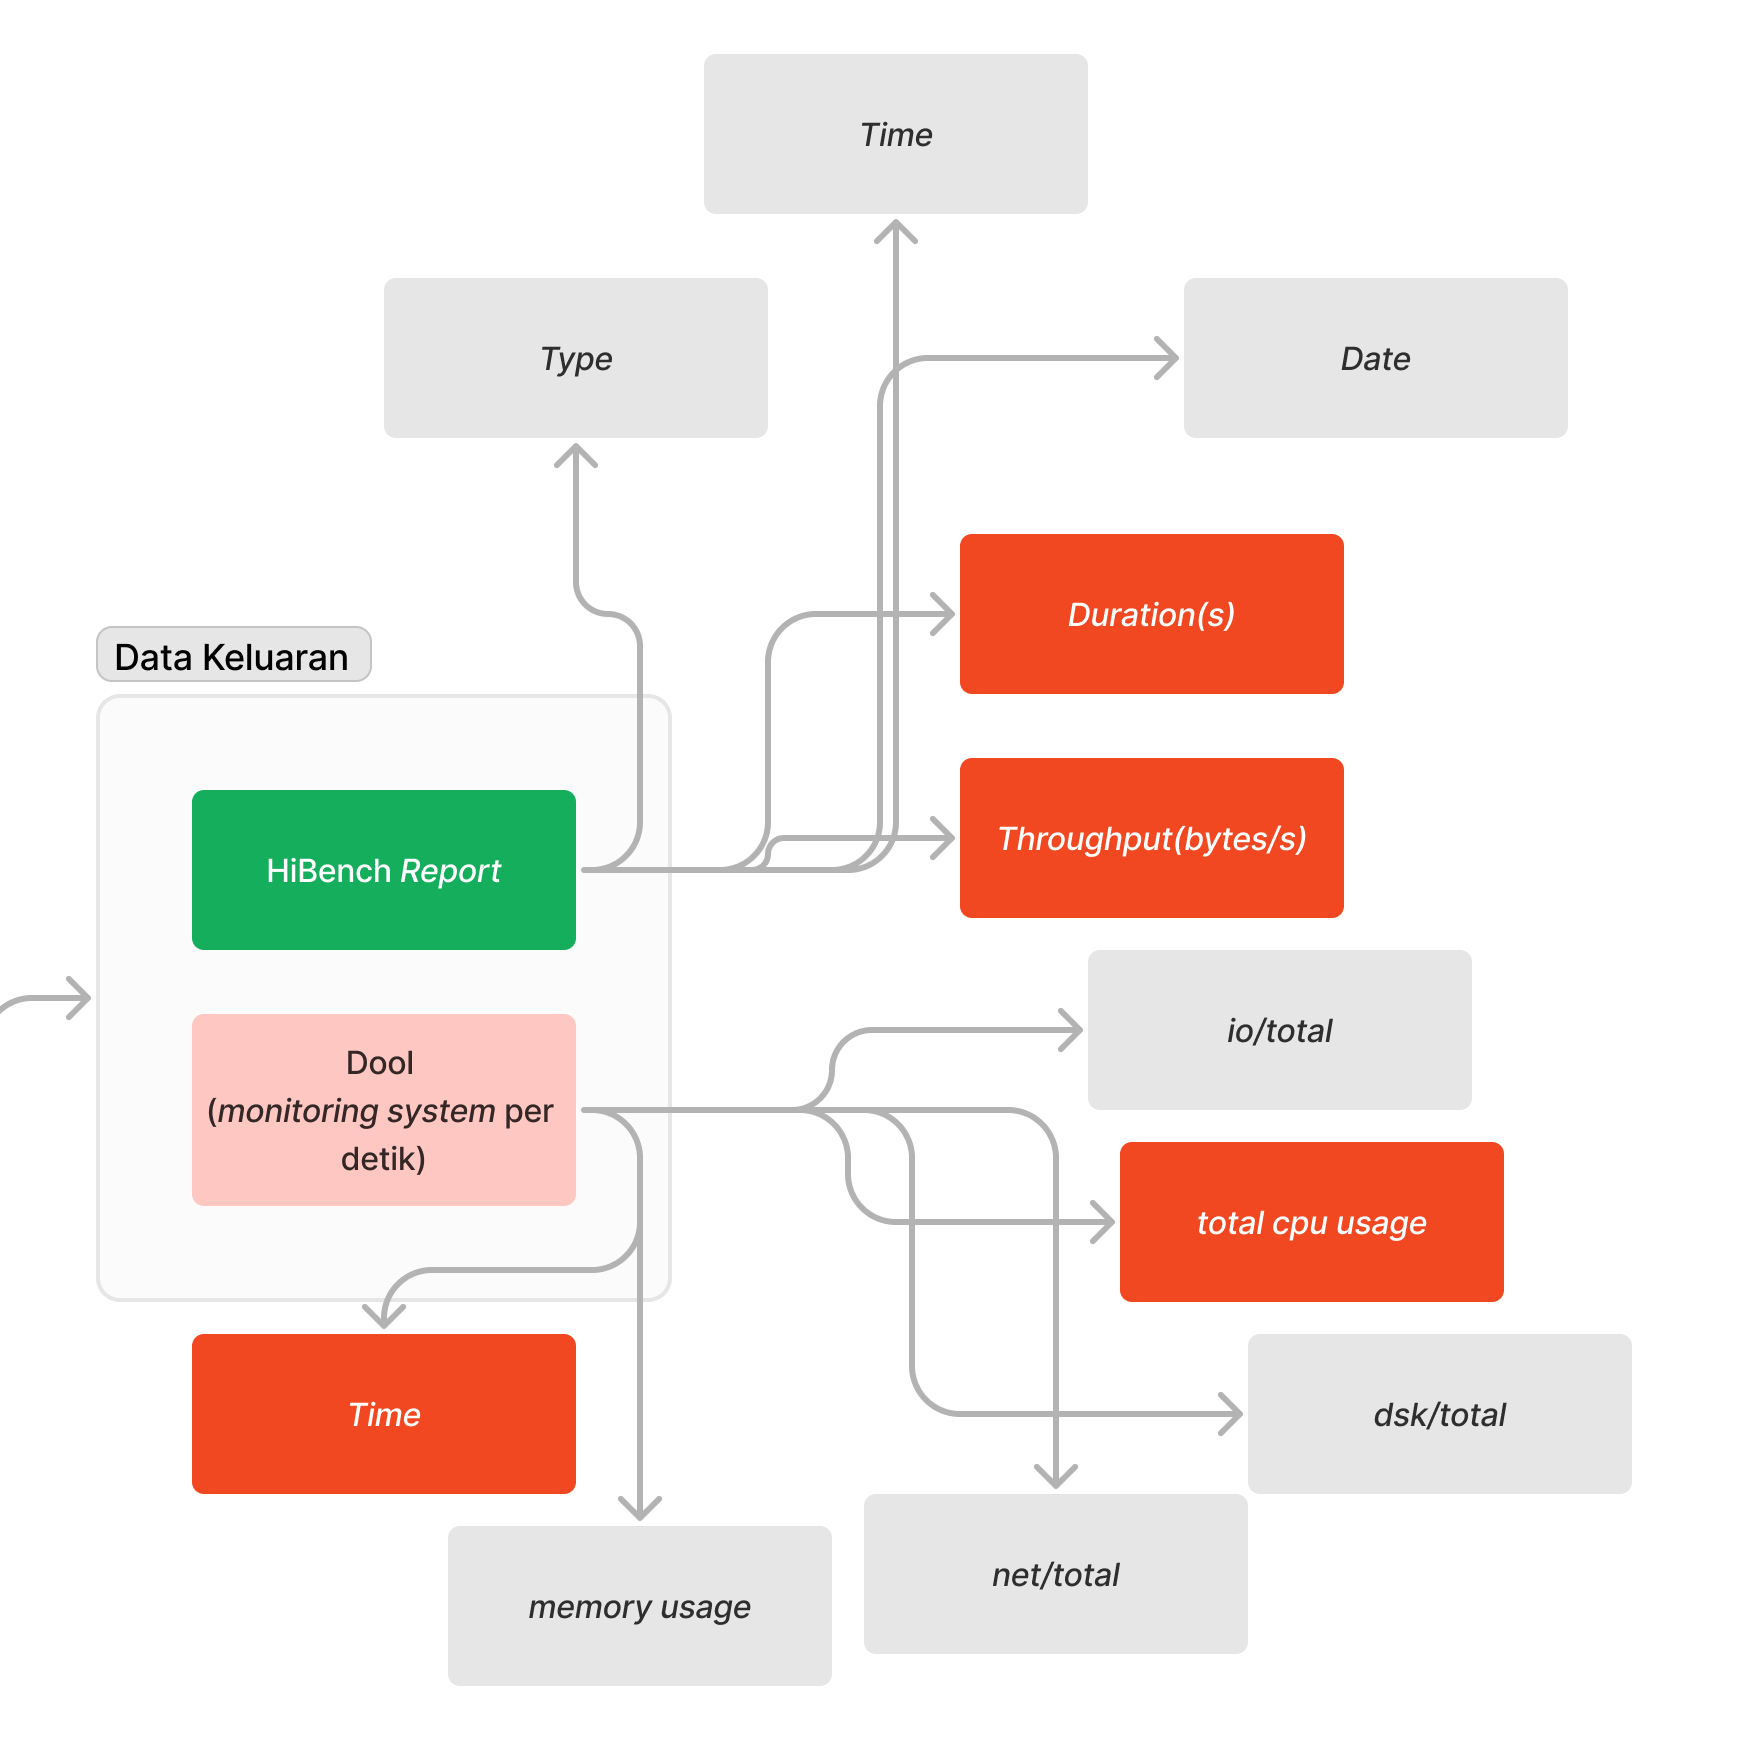
\includegraphics[width=0.9\textwidth]{figures/ch02/output-hibench-dool.png}
    \caption{Data Keluaran HiBench dan Dool}
    \label{fig:output-hibench-dool}
\end{figure}
